\chapter{Outils, Technologies et Architecture Technique}
\label{chap:technologies}

\section{Introduction}

La concrétisation logicielle d'une plateforme d'envergure telle que le \textbf{PMS AMH Hospitality} requiert une sélection rigoureuse d'outils d'ingénierie, de frameworks modernes, de systèmes de gestion de bases de données et d'intergiciels de communication. Face aux exigences critiques de disponibilité, de latence réduite, d'intégrité transactionnelle financière et de sécurité sans mot de passe, chaque brique technologique a été évaluée et intégrée selon des critères de performance industrielle et de pérennité.

Ce chapitre détaille l'ensemble de l'écosystème technologique mobilisé. Nous présenterons successivement les environnements de développement et d'automatisation (Visual Studio Code, Docker Compose, Git/GitHub, SonarQube), les frameworks et langages (FastAPI, Python 3.11, Next.js 14, React 18, TypeScript, Tailwind CSS), la couche de persistance et de messagerie (PostgreSQL 15, Redis 7, RabbitMQ 3.12, MinIO S3), l'architecture des microservices selon le patron \textit{Database per Service}, les spécifications d'API RESTful et enfin l'infrastructure de sécurité Zero-Trust avec Keycloak et le standard WebAuthn/FIDO2.

\section{Environnement de développement et outillage d'ingénierie}

\subsection{Visual Studio Code (IDE)}

La Figure~\ref{fig:logo_vscode} présente l'environnement de développement intégré principal de notre équipe.

\begin{figure}[H]
\centering
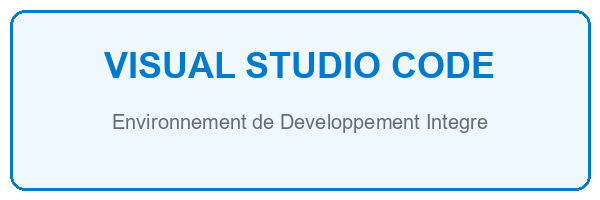
\includegraphics[width=0.55\textwidth]{figures/logo_vscode.png}
\caption{Logo Visual Studio Code}
\label{fig:logo_vscode}
\end{figure}

Visual Studio Code (VS Code) est un éditeur de code source moderne, open-source et multiplateforme développé par Microsoft. Reposant sur le framework Electron et le moteur Monaco Editor, il combine la légèreté d'un éditeur de texte et la puissance d'un IDE complet grâce à son riche écosystème d'extensions.

Dans le cadre du projet PMS AMH, VS Code a été configuré avec les extensions professionnelles suivantes :
\begin{itemize}
    \item \textbf{Python \& Pylance} (Microsoft) : Analyse statique de code, complétion intelligente de type (type hinting), refactoring et navigation rapide dans les symboles de l'application FastAPI ;
    \item \textbf{TypeScript and JavaScript Language Features} : Typage strict, détection d'erreurs en temps réel et IntelliSense sur les composants React 18 / Next.js 14 ;
    \item \textbf{Tailwind CSS IntelliSense} : Autocomplétion des classes d'utilitaires CSS et prévisualisation instantanée des styles ;
    \item \textbf{Docker \& Docker Compose} : Gestion visuelle des conteneurs, inspection des logs en temps réel et exécution de commandes shell dans les conteneurs actifs ;
    \item \textbf{GitLens} : Traçabilité détaillée des commits Git par ligne de code, comparaison de branches et historique visuel des modifications.
\end{itemize}

\subsection{Docker et Docker Compose (Conteneurisation)}

La Figure~\ref{fig:logo_docker} illustre la plateforme de conteneurisation assurant l'isolation et la reproductibilité des environnements.

\begin{figure}[H]
\centering
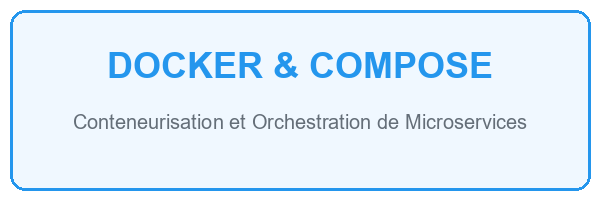
\includegraphics[width=0.55\textwidth]{figures/logo_docker.png}
\caption{Logo Docker et Docker Compose}
\label{fig:logo_docker}
\end{figure}

Docker est une technologie de virtualisation légère au niveau du système d'exploitation (\textit{OS-level virtualization}) qui permet d'encapsuler une application logicielle et l'intégralité de ses dépendances d'exécution (bibliothèques, binaires système, configurations) au sein de conteneurs standardisés, isolés et portables. Docker Compose permet de définir, configurer et orchestrer une architecture multi-conteneurs distribuée à travers un fichier déclaratif unique au format YAML.

Dans notre architecture, Docker Compose coordonne simultanément 18 services conteneurisés interconnectés sur un réseau virtuel privé (\textit{bridge network}) : les 11 microservices backend FastAPI, l'API Gateway Kong, le serveur d'identité Keycloak, l'instance PostgreSQL avec schémas isolés, le serveur Redis 7, le courtier RabbitMQ 3.12, le stockage objet MinIO S3 et le frontend Next.js 14.

\subsection{Git et GitHub (Gestion de versions et CI/CD)}

La Figure~\ref{fig:logo_git} illustre le système de contrôle de versions décentralisé et la plateforme collaborative de développement.

\begin{figure}[H]
\centering
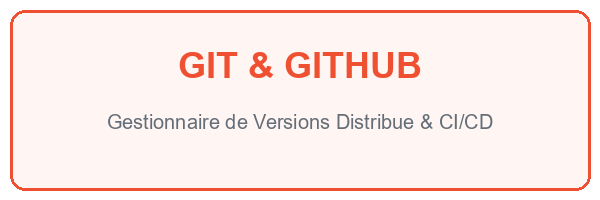
\includegraphics[width=0.55\textwidth]{figures/logo_git.png}
\caption{Logo Git et GitHub}
\label{fig:logo_git}
\end{figure}

Git est un système de gestion de versions décentralisé garantissant l'intégrité cryptographique de l'historique des modifications de code source à travers des arbres de hachage SHA-1/SHA-256. Associé à la plateforme GitHub Enterprise, il a permis de structurer la collaboration au sein de notre équipe d'élèves-ingénieurs selon le modèle du \textit{Feature Branch Workflow} :
\begin{itemize}
    \item La branche \texttt{main} contient le code source de production stable, protégé contre les écritures directes ;
    \item La branche \texttt{develop} centralise les incréments validés de chaque sprint ;
    \item Chaque fonctionnalité nouvelle fait l'objet d'une branche dédiée (ex: \texttt{feature/redis-distributed-lock}, \texttt{feature/webauthn-qr-flow}) soumise à une \textit{Pull Request} (PR) exigeant la validation d'au moins un relecteur et le passage avec succès des tests automatisés avant fusion.
\end{itemize}

\subsection{SonarQube (Audit continu de qualité et de sécurité)}

La Figure~\ref{fig:logo_sonarqube} présente l'outil d'analyse statique continue du code source.

\begin{figure}[H]
\centering
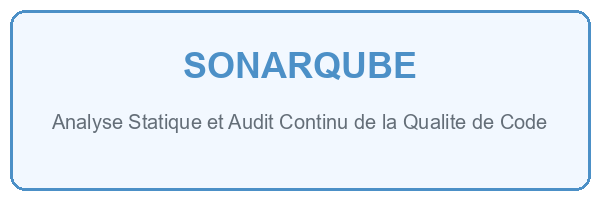
\includegraphics[width=0.55\textwidth]{figures/logo_sonarqube.png}
\caption{Logo SonarQube}
\label{fig:logo_sonarqube}
\end{figure}

SonarQube est une plateforme open-source développée par SonarSource dédiée à l'inspection continue de la qualité du code (\textit{Continuous Code Inspection}). Intégré dans notre pipeline d'intégration continue GitHub Actions, SonarQube analyse le code Python et TypeScript à chaque commit pour vérifier le respect des normes d'ingénierie logicielle, mesurer la dette technique, détecter les failles de sécurité (\textit{Security Hotspots}, injections, fuites de secrets) et certifier le taux de couverture des tests unitaires automatisés.

\section{Frameworks et langages de programmation}

\subsection{FastAPI (Backend Microservices)}

La Figure~\ref{fig:logo_fastapi} illustre le framework web backend moderne retenu pour le projet.

\begin{figure}[H]
\centering
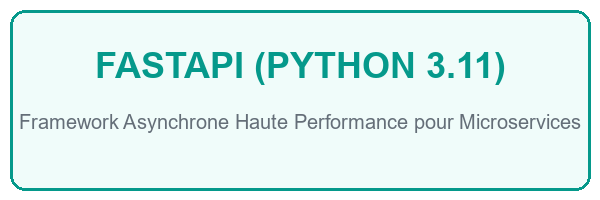
\includegraphics[width=0.55\textwidth]{figures/logo_fastapi.png}
\caption{Logo FastAPI}
\label{fig:logo_fastapi}
\end{figure}

FastAPI est un framework web asynchrone à haute performance développé en Python par Sebastián Ramírez. Fondé sur les composants Starlette (pour le routage ASGI haute vitesse) et Pydantic (pour la validation stricte des données et la sérialisation), FastAPI s'est imposé comme le standard industriel de pointe pour la construction d'API REST distribuées.

Ses atouts décisifs dans le cadre du projet PMS AMH sont :
\begin{itemize}
    \item \textbf{Performances asynchrones natives} : Grâce au support complet des coroutines \texttt{async / await}, FastAPI permet de traiter des milliers de requêtes concurrentes non bloquantes avec une consommation mémoire minimale ;
    \item \textbf{Validation automatique des données} : Les schémas Pydantic valident automatiquement les types et contraintes des payloads JSON entrants (montants financiers, formats de dates, identifiants UUID) et rejettent les requêtes mal formées avec des messages d'erreur explicites (code HTTP 400 ou 422) ;
    \item \textbf{Documentation interactive auto-générée} : FastAPI produit nativement les spécifications OpenAPI 3.0 et expose automatiquement les interfaces interactives Swagger UI (\texttt{/docs}) et ReDoc (\texttt{/redoc}) pour chaque microservice.
\end{itemize}

\subsection{Python 3.11 (Langage Backend)}

La Figure~\ref{fig:logo_python} présente le langage de programmation central de l'architecture microservices.

\begin{figure}[H]
\centering
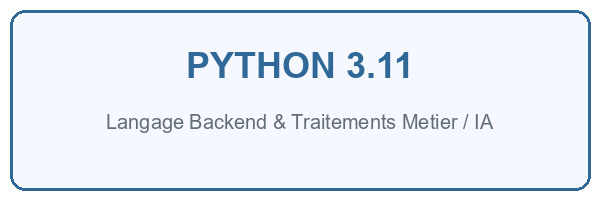
\includegraphics[width=0.55\textwidth]{figures/logo_python.png}
\caption{Logo Python 3.11}
\label{fig:logo_python}
\end{figure}

Python 3.11 apporte des optimisations majeures de performances (moteur d'exécution spécialisé \textit{Adaptive Specializing Interpreter}) réduisant les temps d'exécution de 25\% par rapport aux versions antérieures. Sa clarté syntaxique, sa robustesse pour les calculs mathématiques et fiscaux précis (module \texttt{decimal} évitant les imprécisions des nombres flottants) et la richesse de ses bibliothèques de test (Pytest) en font le langage idéal pour l'ingénierie backend du PMS.

\subsection{Next.js 14 et React 18 (Frontend)}

La Figure~\ref{fig:logo_nextjs} présente le framework React de référence pour les applications web d'entreprise.

\begin{figure}[H]
\centering
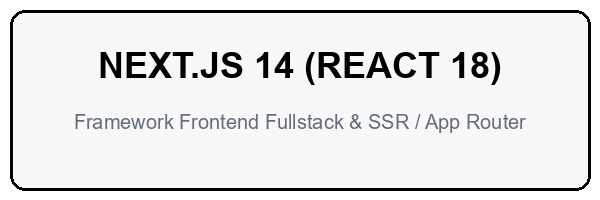
\includegraphics[width=0.55\textwidth]{figures/logo_nextjs.png}
\caption{Logo Next.js 14}
\label{fig:logo_nextjs}
\end{figure}

Next.js 14, développé par Vercel, est un framework fullstack fondé sur React 18. Il introduit l'architecture révolutionnaire de l'\textit{App Router} et des \textit{React Server Components} (RSC), permettant d'exécuter le rendu des composants lourds directement sur le serveur afin d'alléger le bundle JavaScript transmis au navigateur.

Dans le cadre du PMS AMH, Next.js 14 a permis de réaliser :
\begin{itemize}
    \item Un chargement quasi-instantané du tableau de bord d'exploitation grâce au pré-rendu serveur (SSR) ;
    \item Une navigation fluide sans rechargement de page (\textit{Single Page Application}) lors du défilement et des changements de dates sur le planning Tape Chart ;
    \item L'intégration transparente des flux WebSockets pour l'actualisation en temps réel des statuts de chambres et des alertes de réservation.
\end{itemize}

\subsection{TypeScript 5 (Typage Statique Frontend)}

La Figure~\ref{fig:logo_typescript} illustre le langage de développement frontend apportant la rigueur du typage statique.

\begin{figure}[H]
\centering
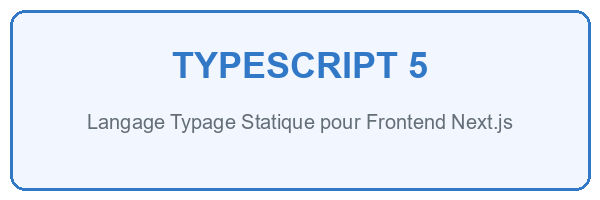
\includegraphics[width=0.55\textwidth]{figures/logo_typescript.png}
\caption{Logo TypeScript 5}
\label{fig:logo_typescript}
\end{figure}

TypeScript, développé par Microsoft, apporte un système de types statiques puissant au-dessus de JavaScript. En garantissant que chaque structure de données manipulée dans le frontend (interfaces \texttt{Booking}, \texttt{Room}, \texttt{Folio}, \texttt{Guest}) corresponde rigoureusement aux schémas JSON renvoyés par les API backend, TypeScript élimine plus de 80\% des erreurs d'exécution classiques (\textit{undefined is not a function}, propriétés manquantes) dès la phase de compilation.

\section{Couche de persistance et intergiciels de communication}

\subsection{PostgreSQL 15 (SGBD Relationnel Transactionnel)}

La Figure~\ref{fig:logo_postgresql} illustre le système de gestion de bases de données relationnelles central de la plateforme.

\begin{figure}[H]
\centering
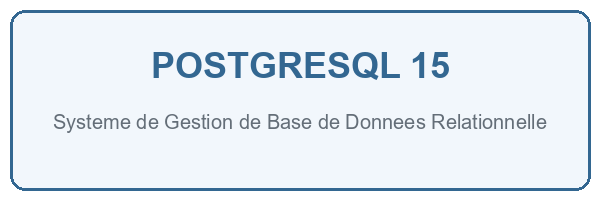
\includegraphics[width=0.55\textwidth]{figures/logo_postgresql.png}
\caption{Logo PostgreSQL 15}
\label{fig:logo_postgresql}
\end{figure}

PostgreSQL 15 est le SGBDR open-source le plus avancé au monde. Réputé pour sa conformité absolue aux propriétés transactionnelles ACID (Atomicité, Cohérence, Isolation, Durabilité), il garantit l'intégrité financière des comptes folios, le respect des clés étrangères et la fiabilité des écritures comptables lors du Night Audit.

Conformément au patron d'architecture \textit{Database per Service}, chaque microservice interagit avec un schéma de base de données dédié et isolé (ex: \texttt{auth\_db}, \texttt{establishment\_db}, \texttt{reservation\_db}, \texttt{billing\_db}), interdisant tout couplage direct par jointures SQL inter-services et imposant une communication exclusive par API REST ou messages AMQP.

\subsection{Redis 7 (Cache en Mémoire et Verrous Distribués)}

La Figure~\ref{fig:logo_redis} présente le magasin de données en mémoire haute vitesse.

\begin{figure}[H]
\centering
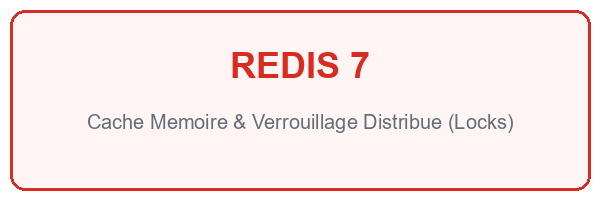
\includegraphics[width=0.55\textwidth]{figures/logo_redis.png}
\caption{Logo Redis 7}
\label{fig:logo_redis}
\end{figure}

Redis 7 est un magasin de données clé-valeur en mémoire offrant des temps de réponse sub-milliseconde. Dans notre architecture, il remplit deux missions critiques :
\begin{enumerate}
    \item \textbf{Mise en cache haute vitesse} des données de référence fréquemment consultées (catalogue des Riads, listes de prix de base) pour soulager la base PostgreSQL ;
    \item \textbf{Gestionnaire de Verrous Distribués (Distributed Lock Manager)} : Implémentation du pattern d'exclusion mutuelle temporaire pour la réservation de chambres. Lors de la sélection d'une chambre par un réceptionniste, le service pose un verrou atomique via la commande :
    \begin{center}
    \texttt{SET lock:room:\{room\_id\}:\{dates\} \{client\_token\} NX PX 10000}
    \end{center}
    Ce verrou, assorti d'un bail temporel (TTL) de 10 secondes, garantit qu'aucun autre opérateur ne peut réserver la même chambre durant la saisie des coordonnées du voyageur, éliminant ainsi toute possibilité d'overbooking.
\end{enumerate}

\subsection{RabbitMQ 3.12 (Bus de Messages Asynchrone AMQP)}

La Figure~\ref{fig:logo_rabbitmq} illustre le courtier de messages assurant le découplage événementiel.

\begin{figure}[H]
\centering

\includegraphics[width=0.55\textwidth]{figures/logo_rabbitmq.png}
\caption{Logo RabbitMQ 3.12}
\label{fig:logo_rabbitmq}
\end{figure}

RabbitMQ est un courtier de messages (\textit{Message Broker}) d'entreprise implémentant le protocole standard AMQP 0-9-1. Il permet d'orchestrer une communication asynchrone et découplée entre les microservices selon le patron de conception \textit{Publish/Subscribe} :
\begin{itemize}
    \item Lorsqu'une réservation est validée, le service Réservation publie un message sur le topic exchange \texttt{pms.events} avec la clé de routage \texttt{booking.created} ;
    \item Le service Housekeeping et le service Notification consomment ce message de manière indépendante et asynchrone pour mettre à jour les plannings d'étage et diffuser les alertes visuelles ;
    \item Les files d'attente durables (\textit{durable queues}) garantissent la persistance des messages sur disque, évitant toute perte de données en cas de redémarrage d'un conteneur.
\end{itemize}

\subsection{MinIO (Stockage Objet Compatible Amazon S3)}

MinIO est un serveur de stockage objet haute performance compatible avec les API Amazon S3. Déployé sous conteneur Docker, il est utilisé pour l'archivage sécurisé et immuable des documents électroniques produits par la plateforme : les rapports d'audit journaliers (\textit{Manager Daily Reports}) et les factures d'hébergement normalisées au format PDF.

\section{Spécifications d'API RESTful et protocoles de communication}

La communication synchrone entre le client Next.js et les microservices backend est régie par les principes architecturaux REST (\textit{Representational State Transfer}) sur protocole HTTPS avec échange de payloads JSON.

Le Tableau~\ref{tab:api_verbs_detail} décrit la sémantique métier des méthodes HTTP mises en œuvre.

\begin{table}[H]
\centering
\small
\renewcommand{\arraystretch}{1.3}
\begin{tabularx}{\textwidth}{|p{2.5cm}|p{4.5cm}|X|}
\hline
\textbf{Méthode} & \textbf{Sémantique Technique} & \textbf{Cas d'Usage Métier dans le PMS AMH} \\
\hline
\textbf{GET} & Lecture sans effet de bord (Idempotente) & Consultation du planning Tape Chart, lecture d'un folio, listing des chambres et fiches clients. \\
\hline
\textbf{POST} & Création de ressource ou déclenchement d'action & Création de réservation, exécution du check-in, enregistrement d'un paiement, lancement du Night Audit. \\
\hline
\textbf{PUT} & Remplacement complet d'une ressource existante & Mise à jour intégrale du profil d'un voyageur ou d'une grille tarifaire. \\
\hline
\textbf{PATCH} & Modification partielle ciblée & Changement du statut ménage d'une chambre (DIRTY $\rightarrow$ CLEAN), modification de dates de séjour. \\
\hline
\textbf{DELETE} & Suppression ou annulation logique & Annulation de réservation, révocation d'une session ou d'une clé d'accès FIDO2. \\
\hline
\end{tabularx}
\caption{Sémantique métier des méthodes HTTP RESTful de la plateforme}
\label{tab:api_verbs_detail}
\end{table}

Le Tableau~\ref{tab:api_codes_detail} récapitule les codes de réponse HTTP normalisés retournés par les microservices.

\begin{table}[H]
\centering
\small
\renewcommand{\arraystretch}{1.3}
\begin{tabularx}{\textwidth}{|p{2.5cm}|p{3.5cm}|X|}
\hline
\textbf{Code HTTP} & \textbf{Intitulé Standard} & \textbf{Signification dans le Contexte Applicatif} \\
\hline
\textbf{200 OK} & Requête traitée avec succès & Données récupérées ou mise à jour partielle réussie. \\
\hline
\textbf{201 Created} & Ressource créée & Nouvelle réservation enregistrée, folio initialisé, charge imputée. \\
\hline
\textbf{204 No Content} & Traitement sans contenu & Suppression ou annulation confirmée avec succès. \\
\hline
\textbf{400 Bad Request} & Requête mal formée & Échec de validation des données d'entrée par Pydantic. \\
\hline
\textbf{401 Unauthorized} & Authentification requise & Jeton JWT absent, corrompu, révoqué ou expiré. \\
\hline
\textbf{403 Forbidden} & Droits d'accès insuffisants & Violation de sécurité RBAC (ex: gouvernante tentant un Night Audit). \\
\hline
\textbf{404 Not Found} & Ressource introuvable & Identifiant de chambre, séjour ou client inexistant dans la base. \\
\hline
\textbf{409 Conflict} & Conflit d'état ou concurrence & Chambre déjà verrouillée par un autre opérateur (anti-overbooking). \\
\hline
\textbf{422 Unprocessable} & Erreur sémantique & Dates d'arrivée postérieures à la date de départ. \\
\hline
\textbf{500 Internal Error} & Erreur interne du serveur & Exception non interceptée lors d'un traitement complexe. \\
\hline
\end{tabularx}
\caption{Matrice des codes de réponse HTTP normalisés}
\label{tab:api_codes_detail}
\end{table}

\section{Outils d'automatisation des tests et validation d'API}

\subsection{Postman (Test et documentation des collections d'API)}

La Figure~\ref{fig:logo_postman} illustre l'outil d'exécution des collections de requêtes API REST.

\begin{figure}[H]
\centering
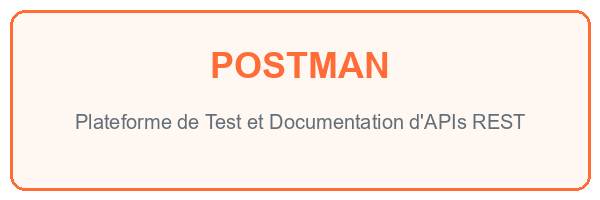
\includegraphics[width=0.55\textwidth]{figures/logo_postman.png}
\caption{Logo Postman}
\label{fig:logo_postman}
\end{figure}

Postman a permis de construire et d'automatiser des suites de tests d'intégration d'API couvrant l'intégralité des 11 microservices, vérifiant la structure des payloads JSON, les codes de statut HTTP et la persistance des en-têtes d'autorisation JWT.

\subsection{Pytest (Framework de tests automatisés backend)}

La Figure~\ref{fig:logo_pytest} présente le framework d'automatisation des tests unitaires en Python.

\begin{figure}[H]
\centering

\includegraphics[width=0.55\textwidth]{figures/logo_pytest.png}
\caption{Logo Pytest}
\label{fig:logo_pytest}
\end{figure}

Pytest, couplé au plugin asynchrone \texttt{pytest-asyncio} et au générateur de couverture \texttt{pytest-cov}, a assuré l'exécution automatisée quotidienne de plus de 140 cas de tests unitaires et d'intégration validant chaque règle de calcul fiscal, transition de statut et verrouillage concurrentiel.

\section{Architecture de sécurité Zero-Trust et protocole WebAuthn}

La sécurité de la plateforme PMS AMH repose sur les principes stricts du modèle Zero-Trust :
\begin{enumerate}
    \item \textbf{Gestion centralisée des identités avec Keycloak} : Serveur IAM open-source assurant la gestion des comptes utilisateurs, des sessions, des politiques de complexité et du cycle de vie des identités ;
    \item \textbf{Contrôle d'accès basé sur les rôles (RBAC)} : Définition de cinq rôles étanches (\texttt{SUPER\_ADMIN}, \texttt{ESTABLISHMENT\_MANAGER}, \texttt{RECEPTIONIST}, \texttt{HOUSEKEEPING}, \texttt{NIGHT\_AUDITOR}) dont les permissions sont injectées sous forme de \textit{claims} dans les jetons JWT signés (RS256) ;
    \item \textbf{Authentification biométrique sans mot de passe WebAuthn / FIDO2} : Standard cryptographique W3C fondé sur la cryptographie à clé publique asymétrique (courbe elliptique ECDSA P-256). L'authentification par scan de QR code sur smartphone personnel élimine radicalement les risques de vol de mot de passe, de phishing et de partage de sessions sur les postes fixes de réception.
\end{enumerate}

\section{Conclusion}

Ce troisième chapitre a exposé l'ensemble des choix d'ingénierie technique et architecturale de la plateforme \textbf{PMS AMH Hospitality}. L'intégration harmonieuse de FastAPI, Python 3.11, Next.js 14, PostgreSQL 15, Redis 7, RabbitMQ 3.12, Docker Compose et Keycloak forme une infrastructure résiliente, modulaire et hautement sécurisée. Le chapitre suivant sera consacré à la phase de réalisation pratique et à la présentation détaillée de l'ensemble des interfaces utilisateurs développées.
